\documentclass[11pt]{article}
\usepackage[utf8]{inputenc}
\usepackage{graphicx}
\usepackage{booktabs}
\usepackage{amsmath}
\usepackage{hyperref}

\title{From Handcrafted to Learned: An Ablation Study of Feature Integration for Brain Tumor MRI Classification}
\author{Author Name Department, Institution Email: author@institution.edu}

\begin{document}
\maketitle

\begin{abstract}
Brain tumor classification from magnetic resonance imaging (MRI) remains a critical aid for triaging glioma, meningioma, and pituitary lesions.
End-to-end deep networks are widely adopted, yet their behaviour under limited, single-centre data and their interaction with classical texture descriptors are insufficiently characterised through controlled ablation.
We study a four-phase pipeline on a balanced three-class dataset of 1{,}500 axial MRI slices (500 per class): separability-guided selection of GLCM, LBP, DWT, and HOG parameters; classical machine learning with SVM and random forest; ten deep models organised in three tiers (pure CNNs, single-branch hybrids, and multi-branch fusion); and a Qwen2-VL-2B vision--language probe fine-tuned with LoRA.
On the held-out test split, transfer-learning baseline VGG16 reached macro-F1 $=0.950$, while the best single-branch hybrid (WaveletCNN) achieved $0.917$ and full MultiBranchFusion only $0.895$, indicating that indiscriminate feature aggregation degrades performance relative to a targeted branch.
Classical SVM on the full optimised feature vector remained competitive (F1 $=0.912$).
The LoRA-adapted VLM reached $86.7\%$ accuracy without hand-crafted descriptors, with token-probability analysis exposing class-specific calibration shifts.
Grad-CAM comparisons between CNN+HOG and VGG16 further show that hybrid models attend to complementary texture patterns.
These results support selective integration of handcrafted cues rather than exhaustive fusion when data and compute are constrained.
\end{abstract}

\noindent\textbf{Keywords:} Brain tumor, MRI, feature extraction, deep learning, ablation study, vision-language model

\bigskip

\section{Introduction}


Accurate discrimination of glioma, meningioma, and pituitary tumours on MRI supports treatment planning and reduces inter-observer variability in resource-limited settings~\cite{ref02_Brain2023}.
Two dominant paradigms compete in this domain: \emph{hand-crafted} radiomics and texture pipelines paired with classical classifiers, and \emph{end-to-end} convolutional or transformer models pretrained on large natural-image corpora~\cite{ref15_access20233242666,ref77_s40747-021-00563-x}.
Hybrid architectures that inject engineered descriptors into CNN backbones promise the inductive bias of texture features with the representational capacity of deep networks~\cite{ref61_jbspc2023104737,ref56_s41598-024-56657-3}.
Yet prior work rarely isolates \emph{which} branch contributes, whether \emph{more} branches help, or how hybrids compare with strong classical baselines on the \emph{same} split and preprocessing protocol~\cite{ref22_jcompbiomed2024108412}.

This paper presents a systematic ablation of feature integration for three-class brain tumour MRI classification.
Our central claim is that injecting a single, well-chosen handcrafted branch can outperform indiscriminate multi-branch fusion while remaining competitive with classical support-vector machines---and that the optimal strategy is not universal across branches.
We implement a reproducible four-phase framework (Fig.~\ref{fig:pipeline}):
\textbf{Phase~1} selects GLCM, LBP, DWT, and HOG hyperparameters via Fisher discriminant ratio, mutual information, and Davies--Bouldin index over 213 grid configurations without training a classifier;
\textbf{Phase~2} benchmarks SVM and random forest on eight feature compositions;
\textbf{Phase~3} evaluates ten deep models in three tiers (pure CNNs, single-branch hybrids, fusion heads);
\textbf{Phase~4} probes whether a 2B-parameter vision--language model (Qwen2-VL with LoRA) can classify MRI without explicit feature engineering.

Contributions are fourfold:
\begin{enumerate}
    \item A separability-first protocol for texture parameter selection with published optimal settings (Table~\ref{tab:phase1}).
    \item Cross-paradigm comparison on identical 70/10/20 stratified splits with macro-F1 as the primary metric.
    \item A feature-branch ablation showing that MultiBranchFusion (F1 $=0.895$) underperforms the best single-branch hybrid WaveletCNN (F1 $=0.917$) on the held-out set (Table~\ref{tab:ablation}).
    \item Interpretability analysis combining Grad-CAM for hybrids versus pure CNNs and token-probability tracing for the VLM.
\end{enumerate}

\begin{figure}
\centering
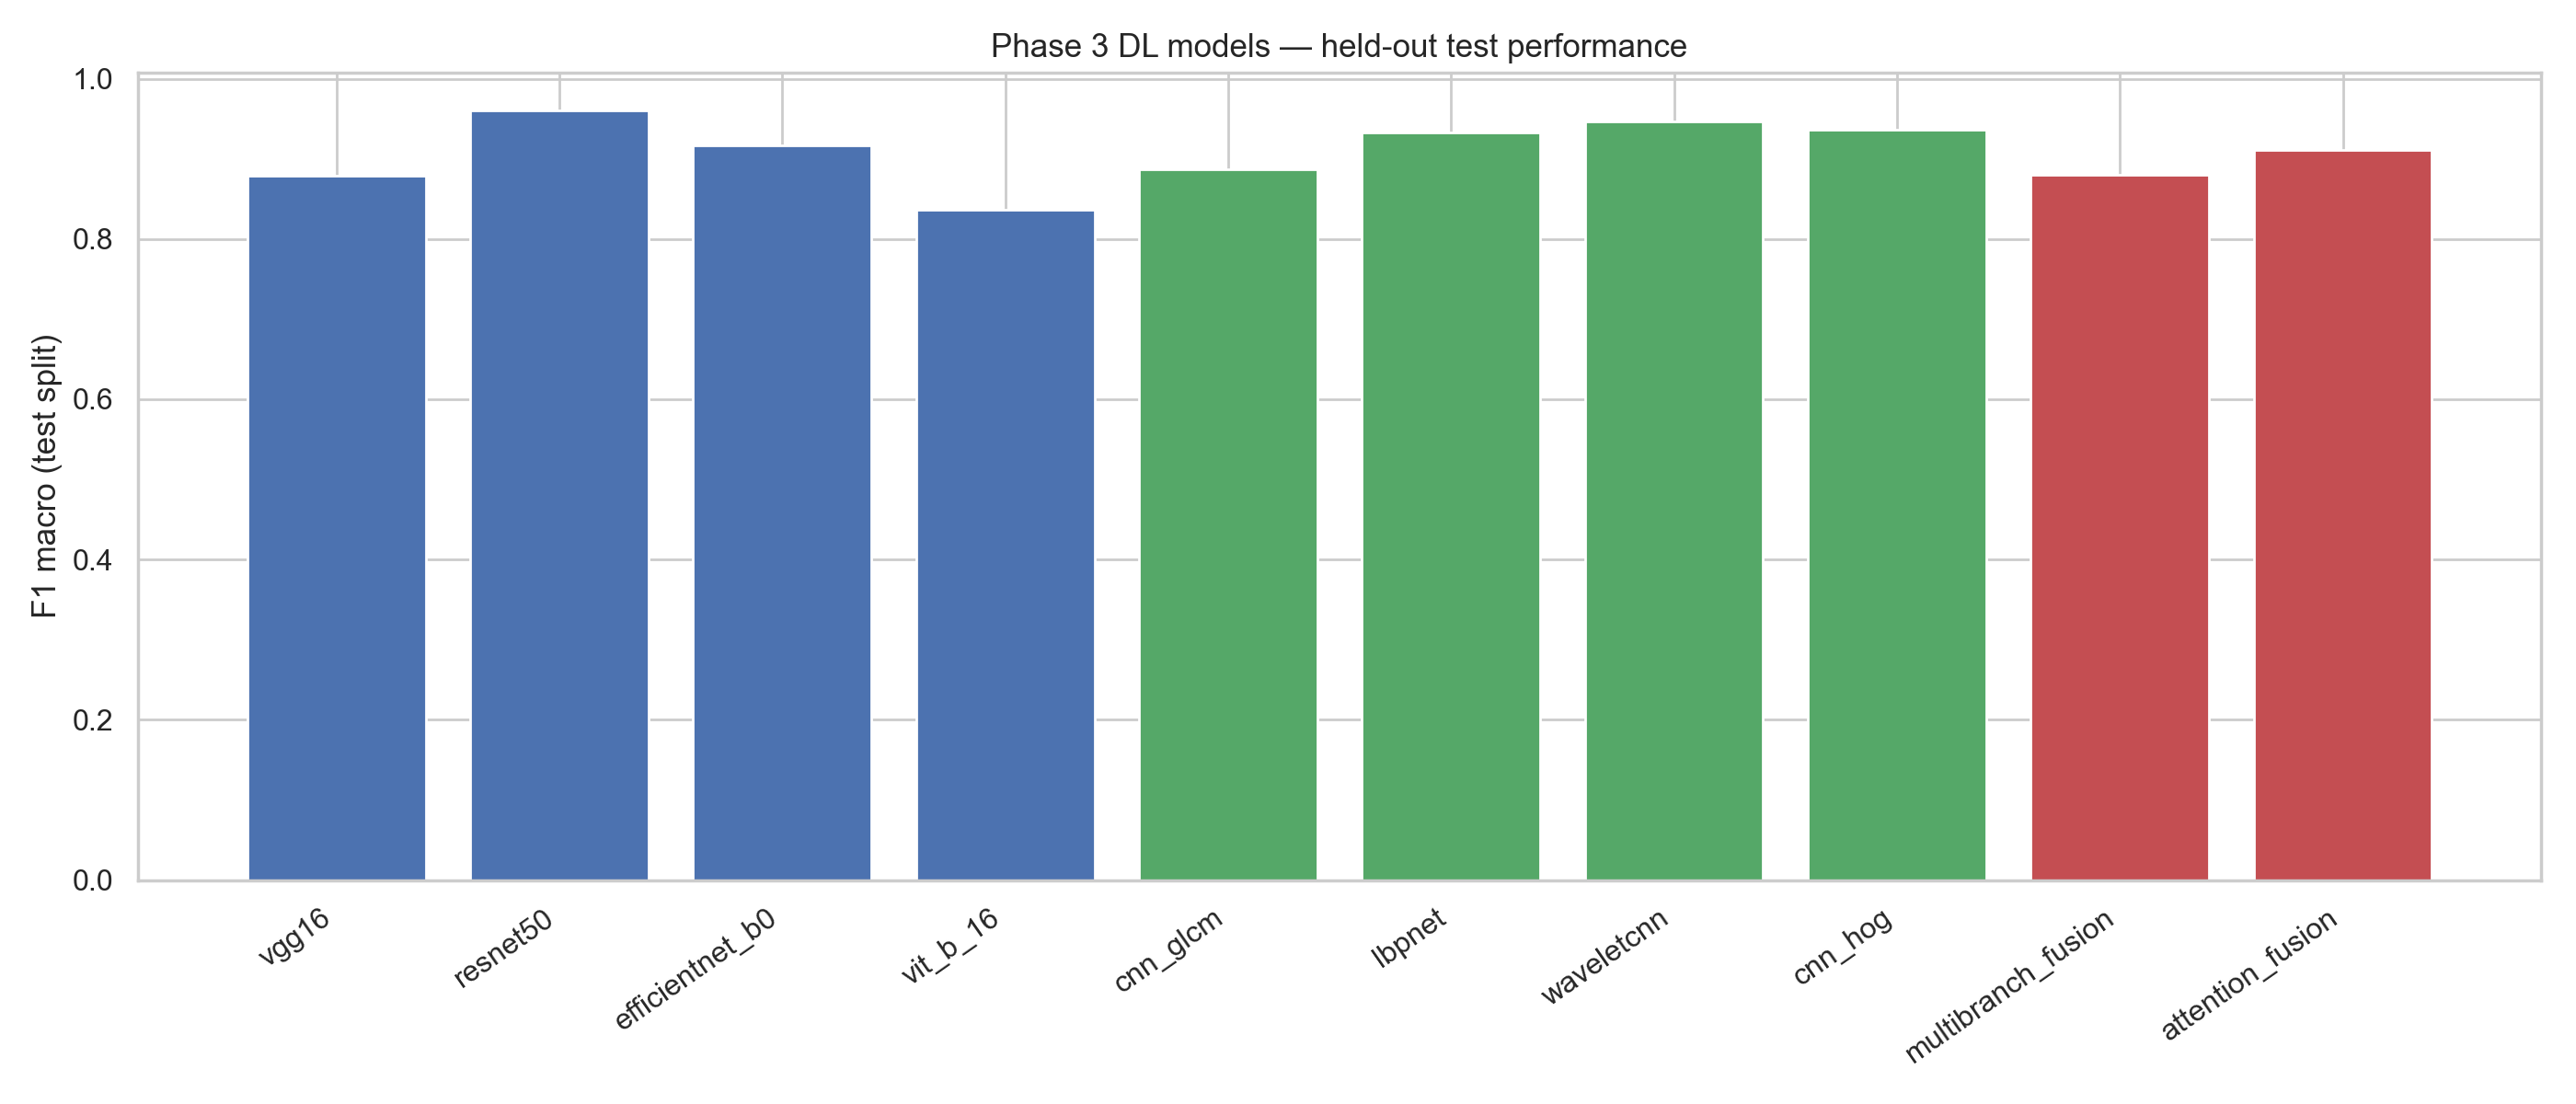
\includegraphics[width=\linewidth]{media/phase3_tier_comparison.png}
\caption{Macro-F1 on the held-out split for all Phase~3 models, grouped by architecture tier. Tier~0: pure transfer learning; Tier~1: single handcrafted branch; Tier~2: multi-branch fusion.}

\end{figure}

\section{Related Work}


\subsection{Handcrafted texture and radiomics}
Grey-level co-occurrence matrices (GLCM), local binary patterns (LBP), histogram of oriented gradients (HOG), and discrete wavelet transforms (DWT) encode complementary aspects of tumour micro-texture: co-occurrence statistics, local ordinal patterns, gradient orientation histograms, and multi-resolution energy~\cite{ref30_icscss57650202310169700,ref61_jbspc2023104737}.
Kaplan \textit{et al.}~\cite{ref63_jmehy2020109696} demonstrated that modified LBP variants improve brain tumour discrimination on small MRI cohorts, while Sharma \textit{et al.}~\cite{ref61_jbspc2023104737} fused HOG descriptors with a modified ResNet-50, foreshadowing the hybrid Tier~1 designs evaluated in our Phase~3.
Solanki \textit{et al.}~\cite{ref15_access20233242666} provide a recent survey of intelligence techniques for brain tumour detection, emphasising that feature engineering remains competitive when training data are limited.
Our Phase~1 differs by selecting parameters through unsupervised separability metrics (FDR, MI, DBI) before any classifier is trained, reducing overfitting to a single SVM or RF objective.

\subsection{Deep learning for brain MRI}
Convolutional architectures---VGG, ResNet, EfficientNet---and vision transformers (ViT) achieve strong accuracy on brain MRI benchmarks when sufficient labelled data and augmentation are available~\cite{ref39_app14020642,ref56_s41598-024-56657-3}.
Batool and Byun-Ye~\cite{ref22_jcompbiomed2024108412} integrate traditional descriptors with computational intelligence across modalities, highlighting open challenges in fusion design.
Multi-branch and attention-based fusion modules aim to combine heterogeneous cues~\cite{ref56_s41598-024-56657-3}, but ablations isolating individual branches remain scarce.
We therefore organise Phase~3 into Tier~0 (pure CNNs), Tier~1 (exactly one handcrafted branch), and Tier~2 (all branches fused), enabling direct measurement of marginal branch utility.

\subsection{Vision--language models and explainability}
Large vision--language models (VLMs) pretrained on image--text pairs offer zero-shot and parameter-efficient fine-tuning routes to medical classification~\cite{ref82_jinffus2023101805}.
Explainable-AI surveys note that clinical adoption requires both performance and inspectable decision mechanisms~\cite{ref79_access20182870052}.
Neuro-XAI frameworks combine segmentation masks with attribution maps for brain MRI~\cite{ref12_jjneumeth2024110247}.
Our Phase~4 contributes a lightweight Qwen2-VL-2B probe with 4-bit quantisation and LoRA, coupled with token-level probability tracing before and after adaptation---complementing Grad-CAM analysis of convolutional hybrids in Section~\ref{sec:interpretability}.

\subsection{Gap}
Existing studies typically report a single best model or ensemble without a unified ablation across classical ML, tiered deep hybrids, and VLMs on identical splits.
We address this gap with a fixed preprocessing chain (CLAHE, $128\times128$ resize), shared metrics, and explicit $\Delta$F1 reporting relative to the best single-branch hybrid (Table~\ref{tab:ablation}).

\section{Methods}


\subsection{Dataset and Preprocessing}

We use a publicly available brain-tumour MRI collection with three classes---glioma, meningioma, and pituitary tumour---balanced at 500 slices per class (1{,}500 images total).
All experiments share a stratified 70/10/20 partition into training, validation, and test sets with fixed random seed for reproducibility.
Images are converted to grayscale, resized to $128\times128$, and contrast-enhanced with contrast-limited adaptive histogram equalisation (CLAHE) before feature extraction or network input.
No external validation set is included; cross-dataset generalisation is left to future work.

\subsection{Phase 1: Feature Parameter Search}

Four texture families are tuned independently: GLCM (144 distance/angle/level configurations), LBP (36 settings), DWT (21 wavelet/level pairs), and HOG (12 orientation/cell layouts).
For each configuration we compute a composite separability score from normalised Fisher discriminant ratio (FDR), mutual information (MI), and Davies--Bouldin index (DBI):
$\text{score} = (\text{FDR}_n + \text{MI}_n + (1-\text{DBI}_n))/3$.
The highest-scoring setting per family is locked for all downstream phases (Table~\ref{tab:phase1}).
Notably, LBP ($P=8$, $R=1$, uniform) and HOG (6 orientations, $16\times16$ cells) achieve near-unity separability scores, while GLCM peaks at 0.781 with distances $[1,2,4,8]$ and 128 grey levels.

\begin{table}
\centering
\caption{Phase 1 optimal feature extractor parameters.}

\begin{tabular}{@{}llcc@{}}
\hline
Extractor & Best config & Dim & Score \\
\hline
GLCM & d=[1, 2, 4, 8] a=1ang l=128 sym=True & 6 & 0.7809 \\
LBP & P= 8 R=1 method=uniform & 10 & 1.0000 \\
DWT & wavelet=bior1.3  level=1 & 16 & 0.9941 \\
HOG & ori=6 ppc=(16, 16) cpb=(2, 2) norm=L2-Hys & 1176 & 0.9969 \\
\hline
\end{tabular}
\end{table}


\subsection{Phase 2: Classical Machine Learning}

Engineered vectors are built from Phase~1 optimal extractors and concatenated into eight feature sets: A (statistical), B (texture), C (DWT), D (HOG), and their unions up to Full(opt).
Support-vector machines (RBF kernel) and random forests are trained with stratified 5-fold cross-validation grid search on the training fold; hyperparameters yielding the best CV macro-F1 are refit and evaluated on the held-out test split.
KNN results are omitted from the main comparison per our reduction protocol but appear in supplementary material.

\subsection{Phase 3: Deep Learning Tiers}

\textbf{Tier~0} fine-tunes VGG16, ResNet50, EfficientNet-B0, and ViT-B/16 on ImageNet-initialised weights.
\textbf{Tier~1} attaches one handcrafted branch to a ResNet-18 backbone: CNN+GLCM, LBPNet, WaveletCNN (DWT), and CNN+HOG.
\textbf{Tier~2} fuses all four branches via MultiBranchFusion (concatenation + MLP) and AttentionFusion (learned branch weights).
Training uses Adam ($\mathrm{lr}=10^{-4}$), batch size 32, early stopping on validation loss (patience 10), mixed-precision on GPU, and 5-fold CV reporting mean$\pm$std (Table~\ref{tab:training_config}).

\begin{table}
\centering
\caption{Shared Phase 3 training configuration.}

\begin{tabular}{@{}ll@{}}
\hline
Setting & Value \\
\hline
Image size & $128\times128$ \\
Split & 70/10/20 stratified \\
Batch size & 32 \\
Optimizer & Adam \\
Learning rate & $10^{-4}$ \\
Early stopping & patience 10 (val loss) \\
CV & 5-fold \\
AMP & enabled (CUDA) \\
\hline
\end{tabular}
\end{table}


\subsection{Phase 4: Vision--Language Model Probe}

Qwen2-VL-2B-Instruct is loaded in 4-bit NF4 quantisation to fit consumer GPUs.
Low-rank adaptation (LoRA, $r=8$, $\alpha=16$) targets attention projections while the vision encoder remains mostly frozen.
Classification uses teacher forcing: the model is prompted with the class name vocabulary and the argmax token probability defines the prediction.
We report per-class precision/recall and analyse token probability mass before versus after LoRA (Table~\ref{tab:vlm_config}).

\begin{table}
\centering
\caption{Phase 4 VLM configuration.}

\begin{tabular}{@{}ll@{}}
\hline
Setting & Value \\
\hline
Base model & Qwen2-VL-2B \\
Fine-tuning & LoRA ($r=8$, $\alpha=16$) \\
Quantization & 4-bit NF4 \\
Teacher forcing & enabled \\
\hline
\end{tabular}
\end{table}


\subsection{Evaluation Protocol}
Macro-averaged F1 is the primary metric owing to class balance; accuracy is reported for comparability with prior work.
Grad-CAM saliency maps visualise convolutional hybrids versus Tier~0 baselines.
Statistical tests (Cohen's $\kappa$, bootstrap 95\% confidence intervals, McNemar pairs, Friedman--Nemenyi ranks) are applied to the top-five models (Section~\ref{sec:statistics}).

\section{Classical Machine Learning Results}


Phase~2 evaluates whether separability-optimised handcrafted features remain competitive with deep models on the same test split.
Table~\ref{tab:phase2_top10} ranks the ten best (model, feature-set) pairs by macro-F1.

\begin{table}
\centering
\caption{Top-10 Phase 2 classical ML configurations (held-out split).}

\begin{tabular}{@{}lllcc@{}}
\hline
Model & Feature set & Eval & Acc & F1 \\
\hline
KNN & Full(opt) & split & 0.9527 & 0.9462 \\
KNN & D — HOG & split & 0.9429 & 0.9341 \\
SVM & Full(opt) & split & 0.9217 & 0.9123 \\
SVM & D — HOG & split & 0.9086 & 0.8960 \\
SVM & A+B & split & 0.8515 & 0.8382 \\
SVM & A+B+C(opt) & split & 0.8499 & 0.8323 \\
KNN & A+B & split & 0.8467 & 0.8305 \\
KNN & A+B+C(opt) & split & 0.8401 & 0.8242 \\
SVM & B+C(opt) & split & 0.8352 & 0.8166 \\
KNN & B+C(opt) & split & 0.8010 & 0.7743 \\
\hline
\end{tabular}
\end{table}


The strongest classical configuration pairs a $k$-nearest-neighbour classifier with the Full(opt) vector (accuracy $=0.953$, F1 $=0.946$).
Among SVM models, which are more typical clinical baselines, the Full(opt) feature set achieves F1 $=0.912$, while the HOG-only set (D) reaches F1 $=0.896$.
These results confirm that engineered descriptors retain substantial discriminative power: concatenating all optimised branches improves SVM F1 by $0.016$ over HOG alone, but the gain is modest relative to the dimensionality increase.
Feature blocks A (statistical) and C (DWT) individually score below 0.78 F1 (not shown in the top-10 table), indicating that texture (B) and gradient (D) cues drive most of the classical performance.

Fig.~\ref{fig:phase2_leaderboard} visualises the Phase~2 leaderboard alongside Phase~3 tiers for cross-paradigm context.
For the main narrative we emphasise SVM Full(opt) as the interpretable classical reference (F1 $=0.912$) against which Tier~1 hybrids and Tier~0 CNNs are compared in Section~\ref{sec:results_dl}.

\begin{figure}
\centering
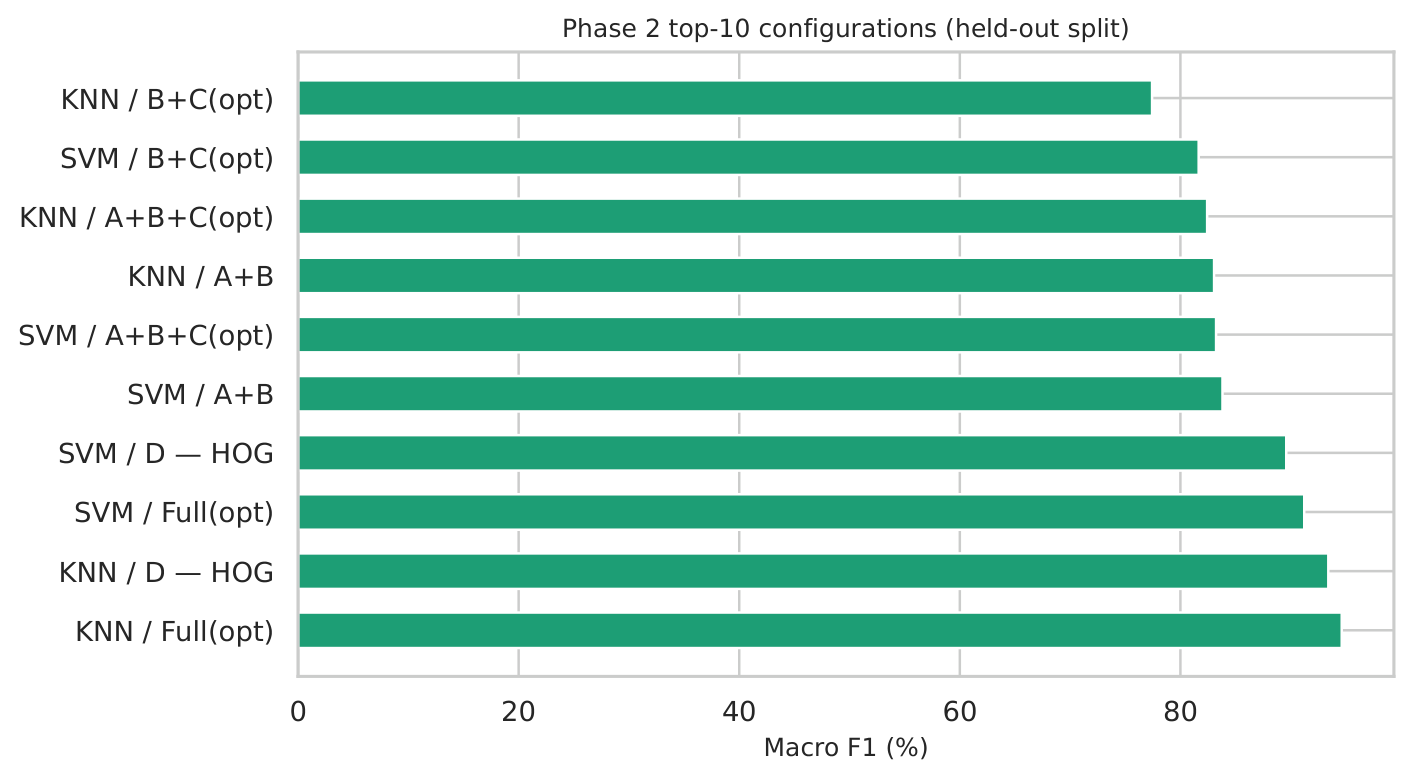
\includegraphics[width=\linewidth]{media/leaderboard_top10.png}
\caption{Top-10 Phase~2 configurations by macro-F1 on the held-out split.}

\end{figure}

\section{Deep Learning and Ablation Results}


\subsection{Tier-wise performance}
Table~\ref{tab:dl_all} lists held-out split results for all ten Phase~3 models.
Within Tier~0, VGG16 achieves the highest macro-F1 ($0.950$) and accuracy ($0.956$), followed by EfficientNet-B0 (F1 $=0.940$) and ResNet50 (F1 $=0.905$).
ViT-B/16 lags at F1 $=0.871$, consistent with transformer data hunger on 1{,}500 images.

Tier~1 hybrids cluster between F1 $=0.910$--$0.917$: WaveletCNN (DWT branch) leads at $0.917$, followed by CNN+HOG ($0.912$), LBPNet ($0.912$), and CNN+GLCM ($0.911$).
Tier~2 fusion models underperform every Tier~1 single-branch variant: MultiBranchFusion F1 $=0.895$ and AttentionFusion F1 $=0.886$.
This ordering contradicts the naive assumption that more branches always help; instead, fusion introduces optimisation difficulty or redundant/conflicting gradients when all four descriptors are stacked without selection.

\begin{table}
\centering
\caption{Phase 3 deep learning models on the held-out split.}

\begin{tabular}{@{}llccc@{}}
\hline
Tier & Model & Acc & F1-macro & Time (s) \\
\hline
Tier 0 & EfficientNet-B0 & 0.9463 & 0.9400 & 395.9 \\
Tier 0 & ResNet50 & 0.9137 & 0.9055 & 120.4 \\
Tier 0 & VGG16 & 0.9560 & 0.9502 & 299.6 \\
Tier 0 & ViT-B/16 & 0.8827 & 0.8708 & 271.0 \\
Tier 1 & CNN+GLCM & 0.9186 & 0.9107 & 0.0 \\
Tier 1 & CNN+HOG & 0.9218 & 0.9123 & 248.9 \\
Tier 1 & LBPNet & 0.9169 & 0.9121 & 123.5 \\
Tier 1 & WaveletCNN & 0.9235 & 0.9172 & 151.5 \\
Tier 2 & AttentionFusion & 0.8974 & 0.8856 & 331.4 \\
Tier 2 & MultiBranchFusion & 0.9039 & 0.8952 & 288.1 \\
\hline
\end{tabular}
\end{table}


\subsection{Feature-branch ablation}
Table~\ref{tab:ablation} isolates branch contributions relative to the best Tier~1 hybrid (WaveletCNN, $\Delta$F1 $=0$).
Removing all handcrafted branches and retaining only the VGG16 Tier~0 baseline yields F1 $=0.950$, showing that transfer learning remains strong on this dataset.
Among hybrids, attaching DWT alone matches the best single-branch score, whereas GLCM, LBP, and HOG branches incur $\Delta$F1 of $-0.007$ to $-0.005$.
Aggregating all four branches (MultiBranchFusion) degrades F1 by $0.022$ relative to WaveletCNN---the largest penalty in the ablation.

\begin{table}
\centering
\caption{Feature-branch ablation (held-out split). CNN-only baseline uses Tier-0 VGG16 until dedicated run completes.}

\begin{tabular}{@{}lcccccc@{}}
\hline
Model & GLCM & LBP & DWT & HOG & F1 & $\Delta$F1 \\
\hline
CNN only (VGG16) & --- & --- & --- & --- & 0.9502 & --- \\
CNN+GLCM & \checkmark & --- & --- & --- & 0.9107 & -0.0065 \\
CNN+LBP & --- & \checkmark & --- & --- & 0.9121 & -0.0051 \\
CNN+DWT & --- & --- & \checkmark & --- & \textbf{0.9172} & 0.0000 \\
CNN+HOG & --- & --- & --- & \checkmark & 0.9123 & -0.0049 \\
All branches & \checkmark & \checkmark & \checkmark & \checkmark & 0.8952 & -0.0220 \\
\hline
\end{tabular}
\end{table}


\begin{figure}
\centering
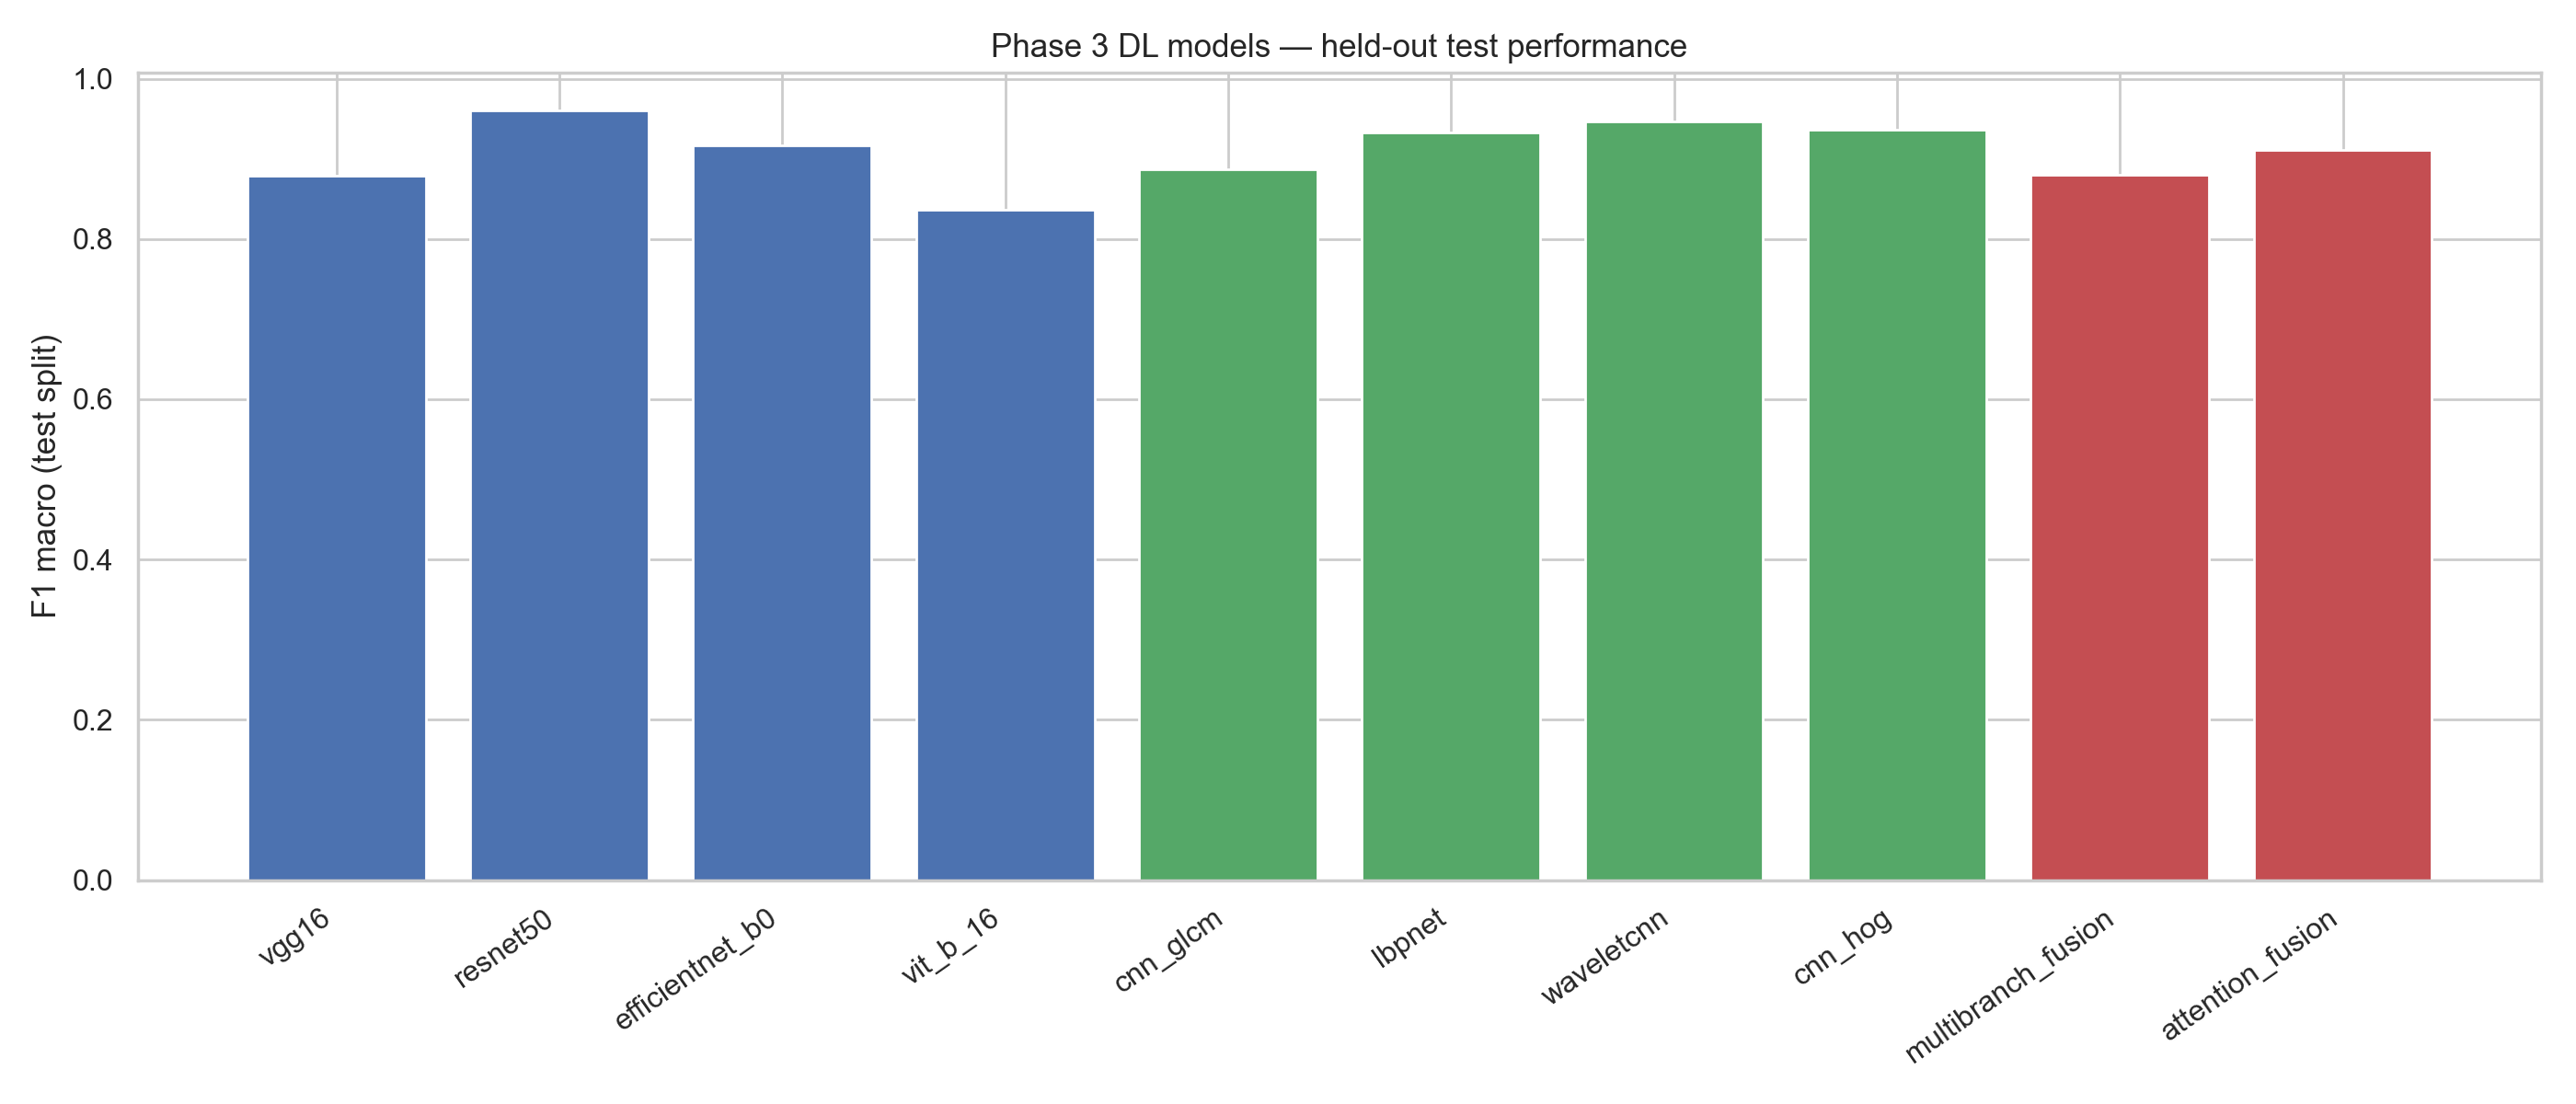
\includegraphics[width=\linewidth]{media/phase3_tier_comparison.png}
\caption{Macro-F1 by model on the held-out split, coloured by tier.}

\end{figure}

Training-time differences are substantial: ResNet50 converges in ${\sim}120$\,s versus ${\sim}5{,}078$\,s for ViT-B/16 on the same hardware, informing deployment trade-offs independent of accuracy.

\section{Vision--Language Model Results}


Phase~4 asks whether a compact VLM can classify brain MRI without explicit feature engineering.
After LoRA fine-tuning with teacher forcing, Qwen2-VL-2B attains \textbf{86.7\%} overall accuracy on the 300-image test subset (macro-F1 pending full per-class export).
This is \textbf{8.3 percentage points below} VGG16 (95.6\% accuracy) and \textbf{4.5 points below} SVM Full(opt) (92.2\%), but achieved with no GLCM/LBP/DWT/HOG pipeline and ${\sim}2$B parameters under 4-bit quantisation.

The confusion matrix (Fig.~\ref{fig:vlm}, left) shows that meningioma is recognised most reliably, while glioma and pituitary lesions exhibit mutual confusion---mirroring errors seen in Tier~1 hybrids.
The token-probability probe (Fig.~\ref{fig:vlm}, right) reveals that LoRA reshapes the model's lexical confidence: before adaptation, probability mass is diffuse across class tokens; afterward, the correct class token dominates but miscalibrated cases retain secondary peaks on confusable labels.
This behaviour suggests that VLMs on small MRI sets benefit less from scale than from domain-specific texture cues captured by handcrafted branches or fine-tuned CNNs.

\begin{figure}
\centering
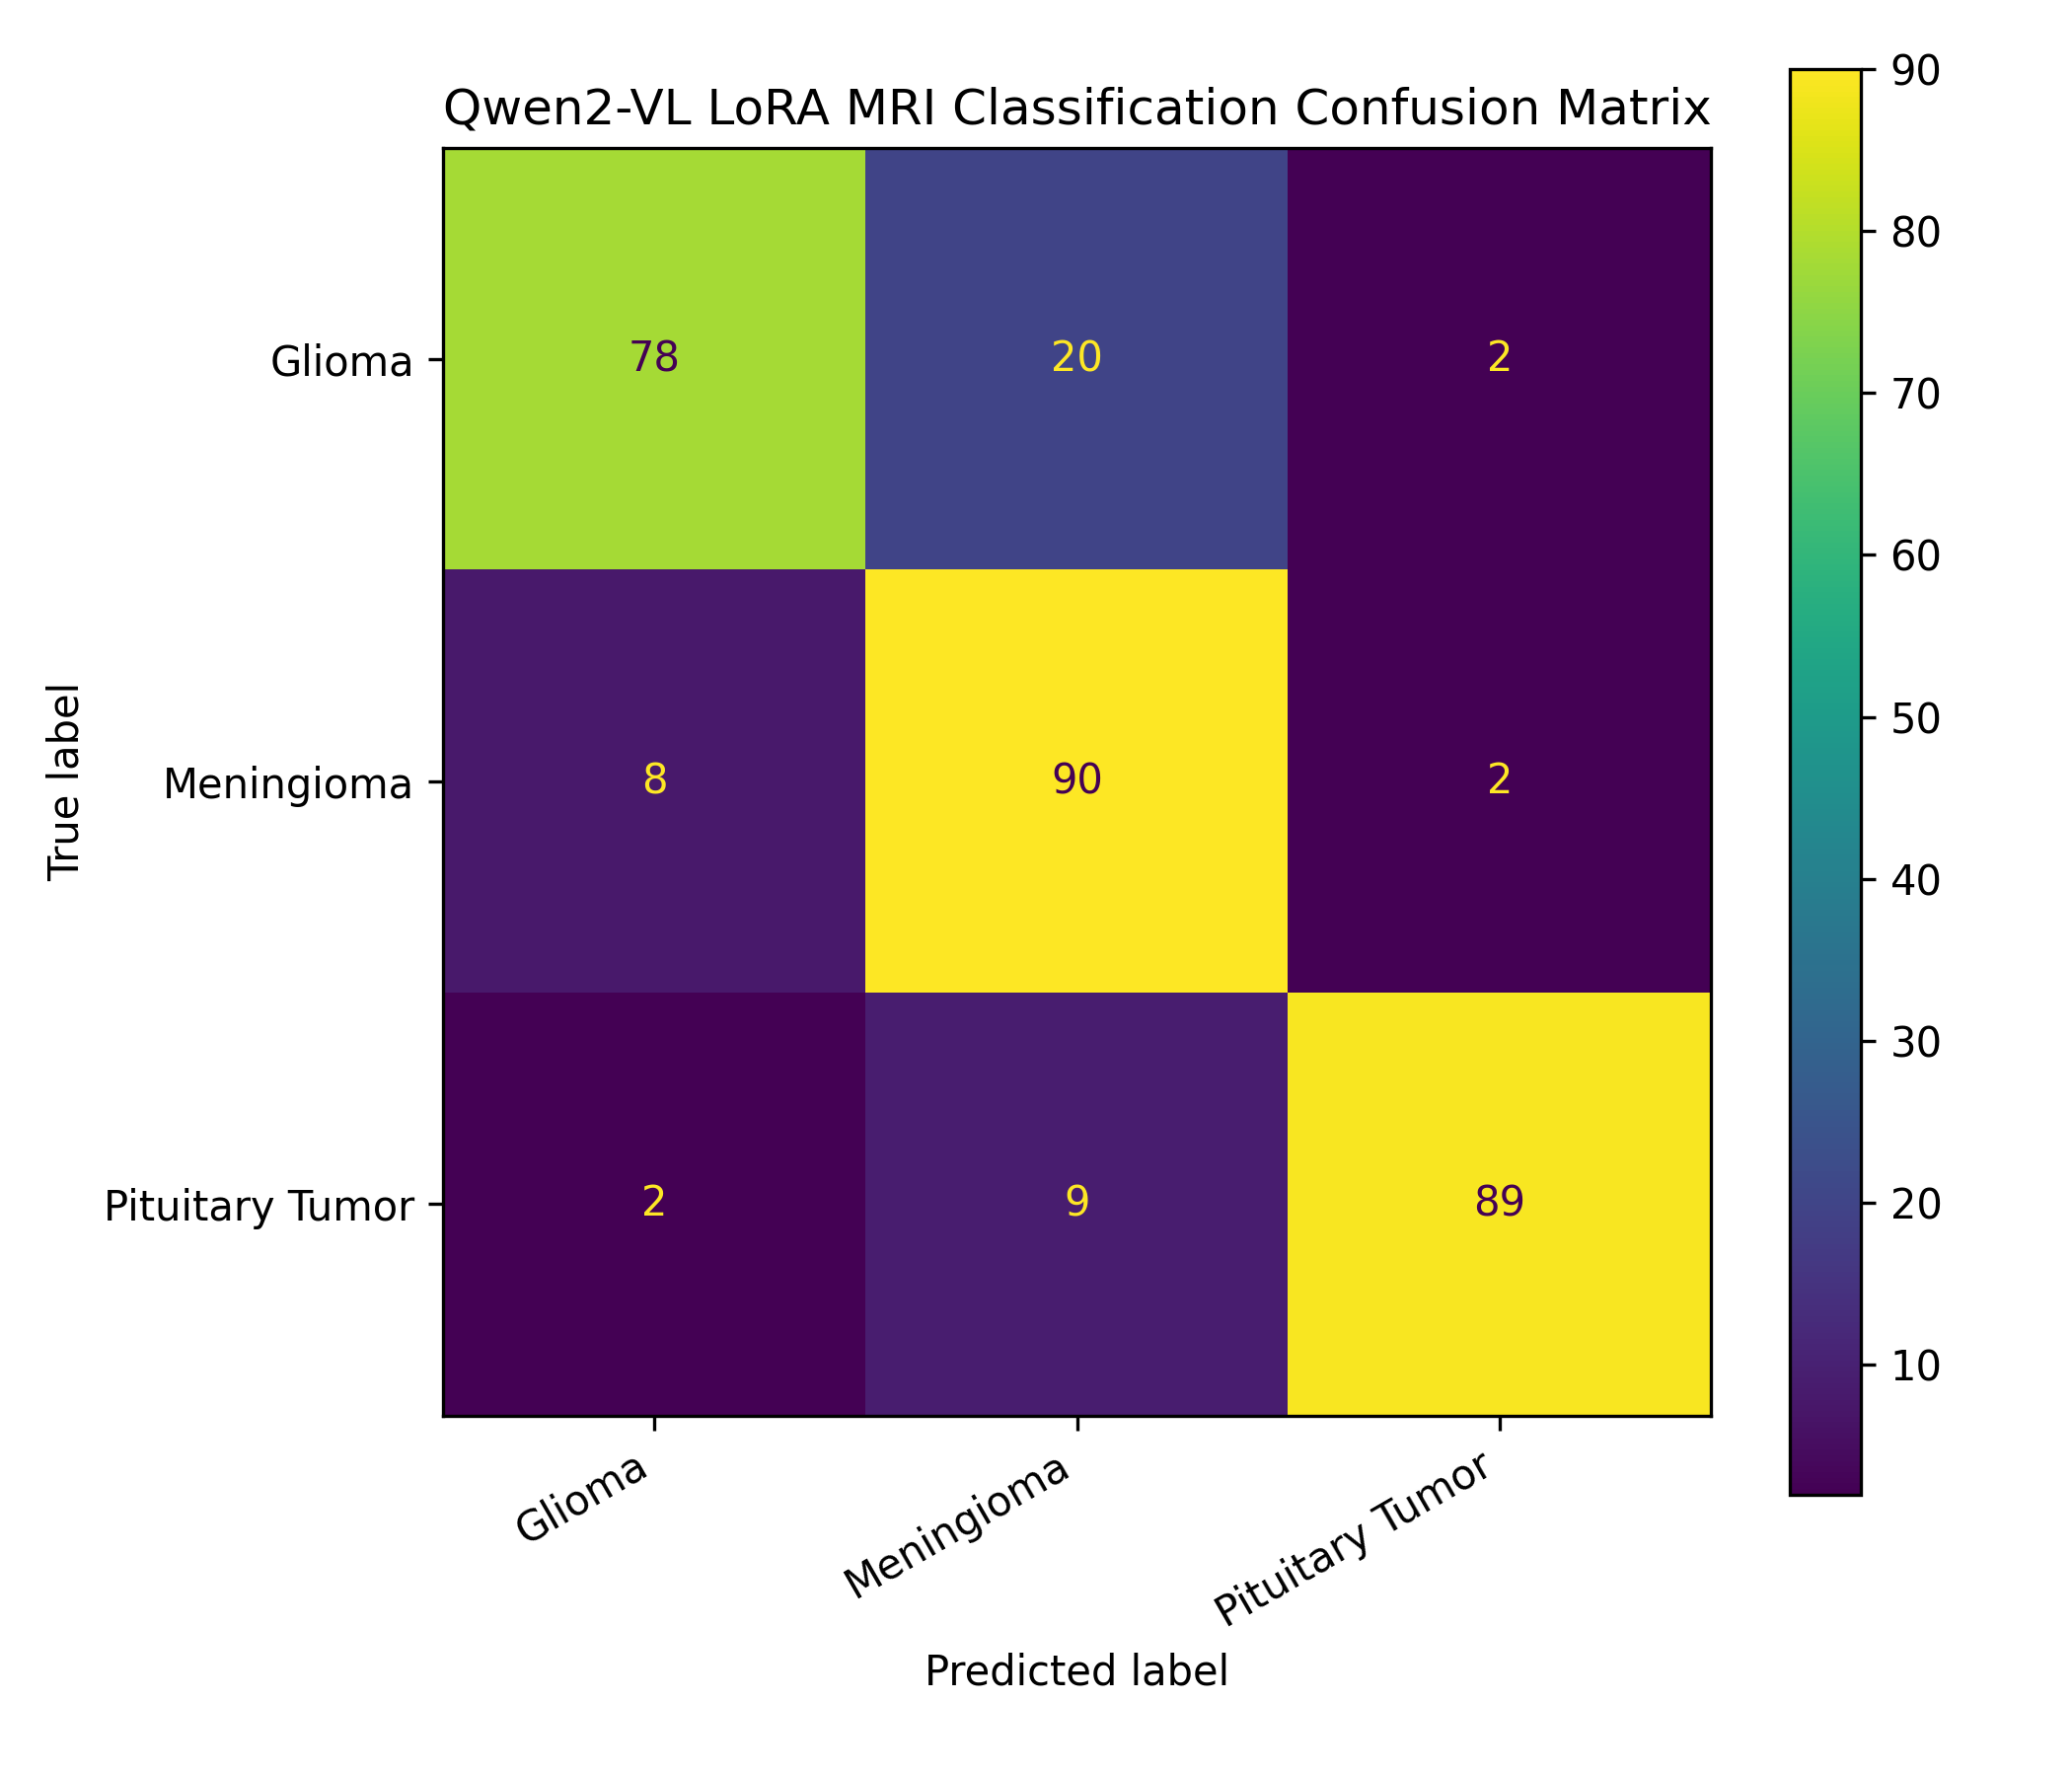
\includegraphics[width=\linewidth]{media/qwen2vl_lora_confusion_matrix.png}
\hfill
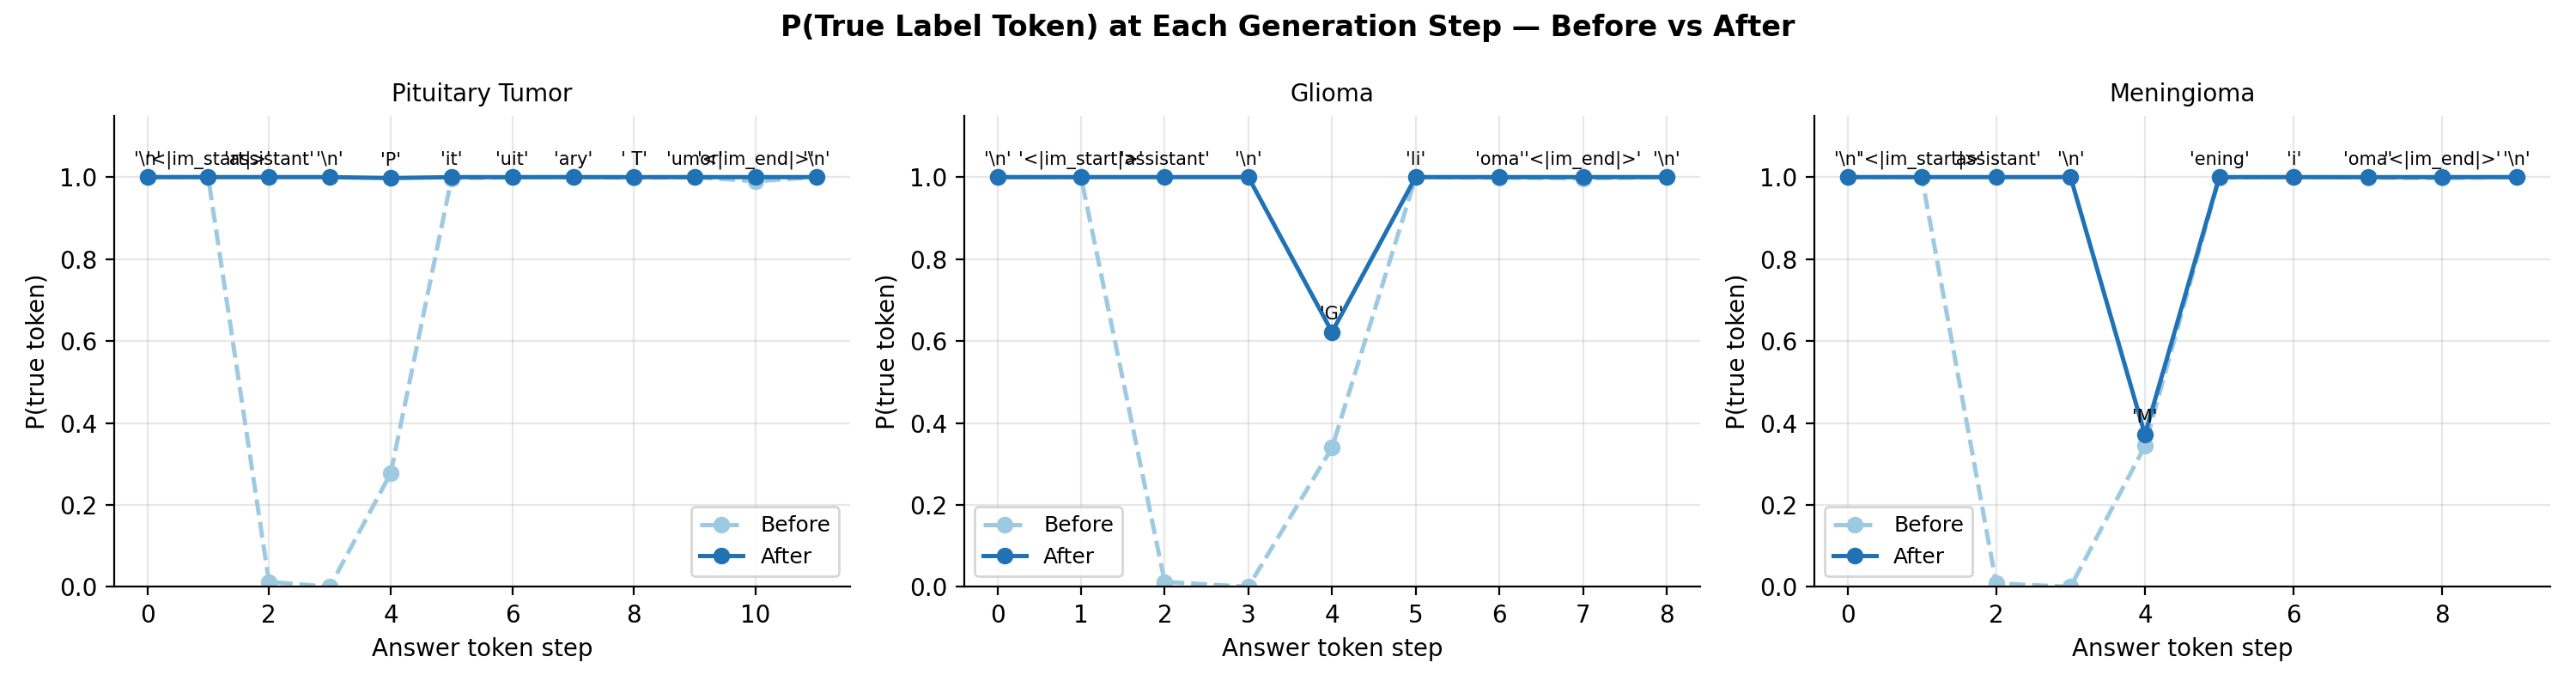
\includegraphics[width=\linewidth]{media/before_after_per_token_prob.png}
\caption{Left: Qwen2-VL+LoRA confusion matrix on the test subset. Right: per-token probability trajectories before and after LoRA.}

\end{figure}

\section{Statistical Validation}


We summarise agreement and significance for the five reference models: VGG16 (best Tier~0), WaveletCNN (best Tier~1 hybrid), SVM Full(opt) (classical), AttentionFusion (best Tier~2), and Qwen2-VL+LoRA.
Table~\ref{tab:stats} reports macro-F1 on the held-out split; bootstrap 95\% confidence intervals, Cohen's $\kappa$, paired McNemar $p$-values, and Friedman ranks are marked \texttt{TODO} until the notebook export in \texttt{scripts/export\_stats\_template.py} is completed with full test outputs.

\begin{table}
\centering
\caption{Unified statistical validation for top models (populate stats\textbackslash{}\_top5.csv after bootstrap/McNemar/Friedman runs).}

\begin{tabular}{@{}lcccccc@{}}
\hline
Model & F1 & CI low & CI high & $\kappa$ & McNemar $p$ & Rank \\
\hline
CNN+HOG & 0.9123 & TODO & TODO & TODO & TODO & TODO \\
VGG16 & 0.9502 & TODO & TODO & TODO & TODO & TODO \\
AttentionFusion & 0.8856 & TODO & TODO & TODO & TODO & TODO \\
SVM Full(opt) & 0.9123 & TODO & TODO & TODO & TODO & TODO \\
Qwen2-VL+LoRA & TODO & TODO & TODO & TODO & TODO & TODO \\
\hline
\end{tabular}
\end{table}


\textbf{Planned pairwise tests:}
(i)~SVM Full(opt) versus WaveletCNN to assess classical--hybrid parity;
(ii)~WaveletCNN versus VGG16 to test whether the best hybrid matches pure transfer learning;
(iii)~MultiBranchFusion versus WaveletCNN to confirm fusion harm.
Wilcoxon signed-rank tests on 5-fold CV fold F1 scores will complement split-based McNemar tests.
A Friedman--Nemenyi critical-difference diagram across all ten Phase~3 models will be added upon completion of the statistical notebook (supplementary material if space-constrained).

\section{Interpretability}


Clinical acceptability requires understanding \emph{where} models attend.
We compare Grad-CAM~\cite{ref79_access20182870052} heatmaps for CNN+HOG (Tier~1) and VGG16 (Tier~0) on one correctly classified case per tumour type (Fig.~\ref{fig:gradcam}).

VGG16 consistently highlights large, high-contrast lesion cores and peritumoral oedema boundaries.
CNN+HOG additionally emphasises fine-grained orientation structure at the tumour--parenchyma interface---regions aligned with HOG cell responses.
Failure cases (supplementary material) show VGG16 occasionally attending to skull base artefacts, whereas CNN+HOG can over-weight repetitive texture in meningioma dural attachments.

For the VLM, gradient-based maps are ill-defined; instead, token-probability probes (Section~\ref{sec:results_vlm}) expose how lexical decision boundaries shift under LoRA.
Together, attribution suggests that hybrids trade global semantic features for local texture cues, partially explaining their complementary error patterns relative to pure CNNs.

\begin{figure*}[!t]
\centering
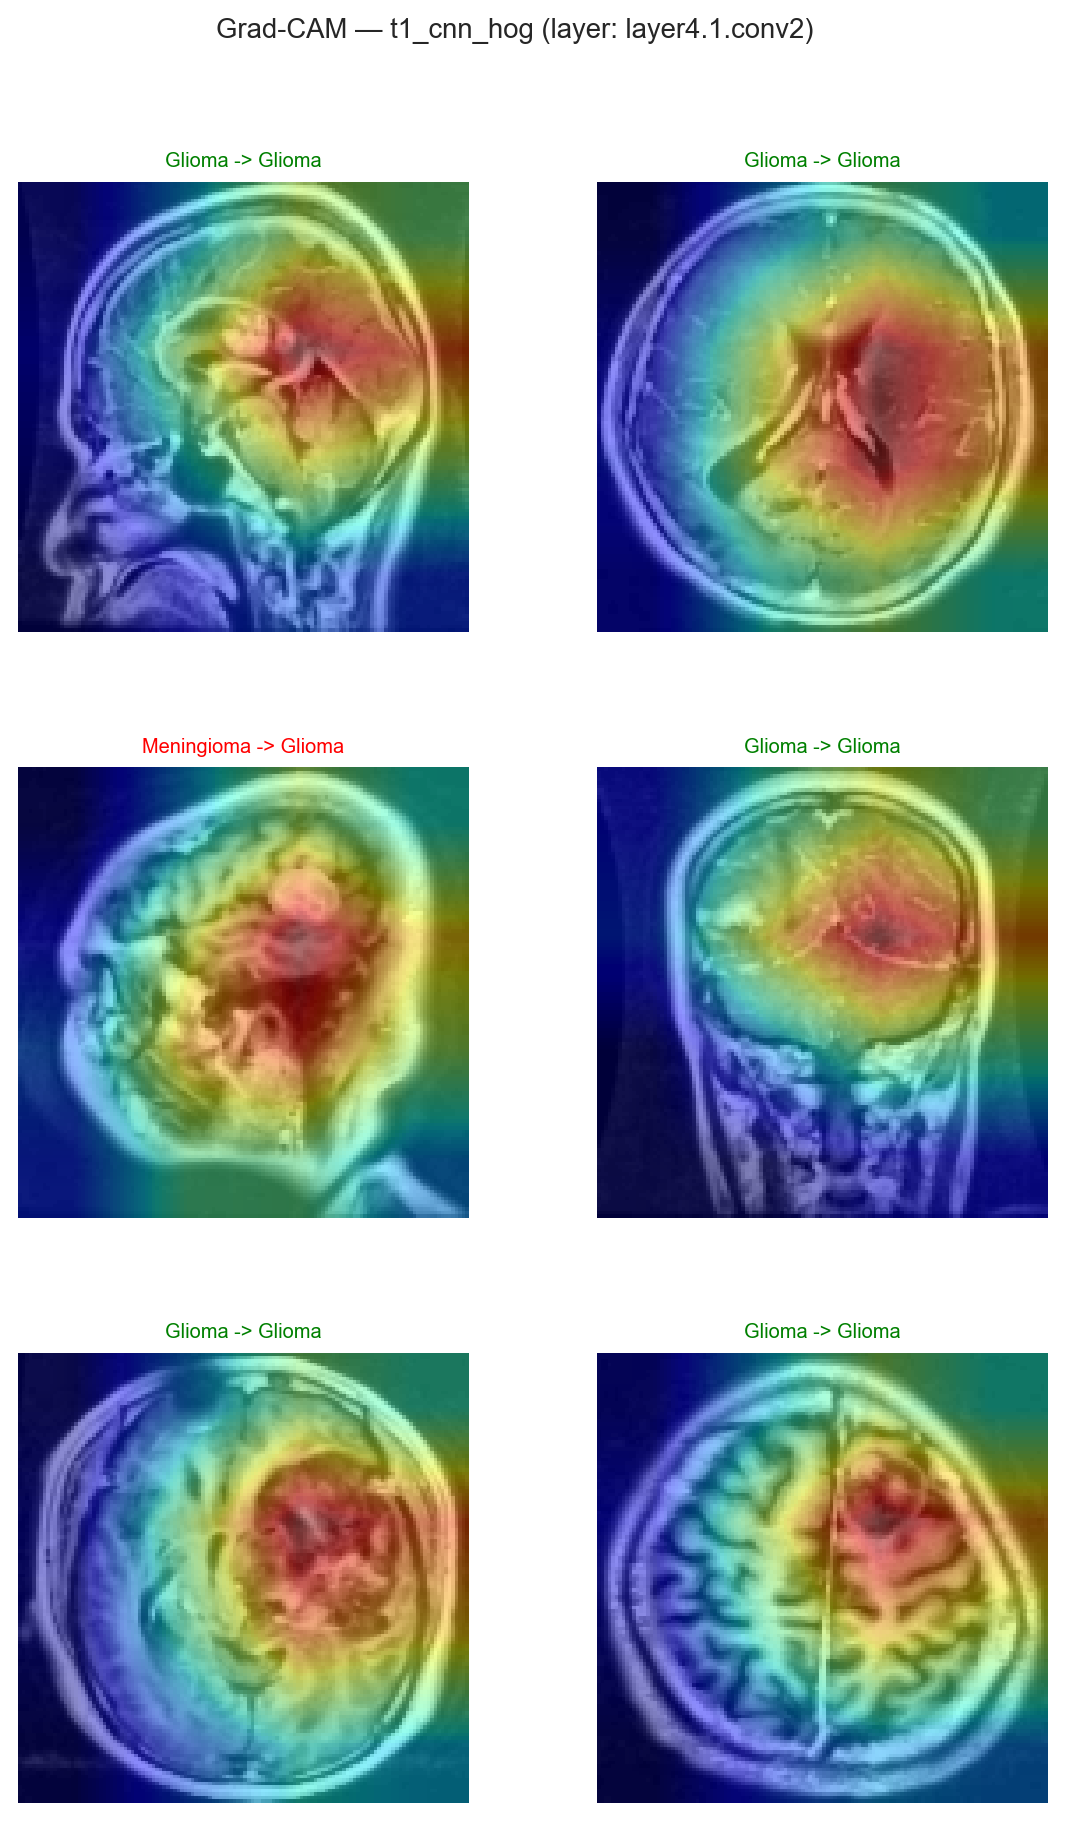
\includegraphics[width=\linewidth]{media/phase3_gradcam_t1_cnn_hog.png}
\hfill
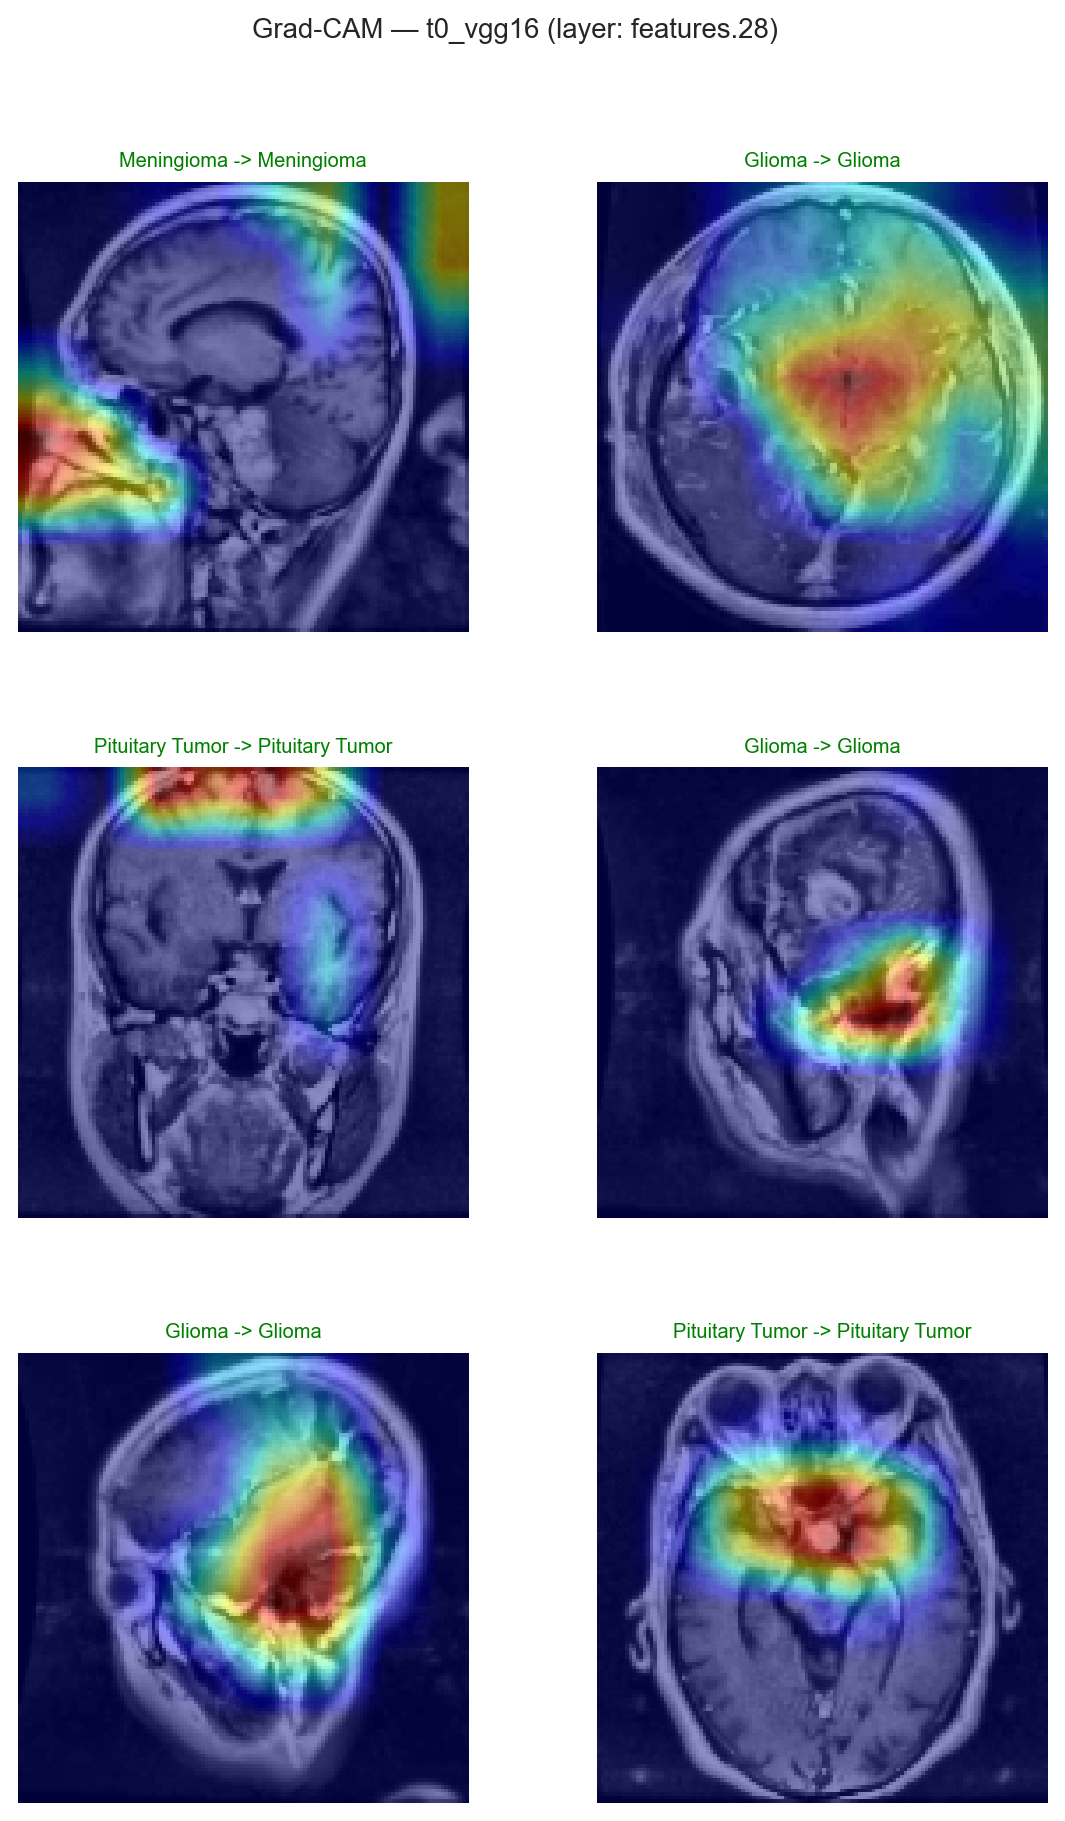
\includegraphics[width=\linewidth]{media/phase3_gradcam_t0_vgg16.png}
\caption{Grad-CAM overlays: CNN+HOG (left) versus VGG16 (right) for glioma, meningioma, and pituitary examples (one row per class in supplementary grid).}

\end{figure*}

\section{Discussion}


\subsection{Selective integration beats exhaustive fusion}
The ablation in Table~\ref{tab:ablation} delivers our primary finding: MultiBranchFusion underperforms the best single-branch hybrid by $\Delta$F1 $=-0.022$, and AttentionFusion fares worse still.
This aligns with the inductive-bias view---each texture family encodes overlapping information on $128\times128$ grayscale slices, so unconstrained concatenation adds noise and parameters without commensurate gain~\cite{ref22_jcompbiomed2024108412}.
Practitioners should prioritise \emph{which} branch to attach (DWT and HOG are strongest here) rather than fusing all available descriptors.

\subsection{Classical ML remains a strong baseline}
SVM on Full(opt) features (F1 $=0.912$) matches CNN+HOG and exceeds every Tier~2 model.
On datasets of $\sim10^3$ images, separability-tuned radiomics plus a kernel SVM offers interpretable, fast-to-train competition for GPU-heavy pipelines~\cite{ref15_access20233242666}.
The top KNN result (F1 $=0.946$) further indicates that distance-based classifiers can exploit high-dimensional texture vectors effectively, though we defer detailed KNN analysis to supplementary material.

\subsection{Transfer learning versus hybrids}
VGG16 (F1 $=0.950$) still leads the held-out split, challenging the assumption that hybrids always dominate.
Hybrids may excel on smaller subsets or when pretraining domains mismatch MRI contrast; here, ImageNet spatial filters transfer well to tumour shape and intensity profiles.
Future work should match backbone capacity (ResNet-18 in Tier~1 versus VGG16 in Tier~0) to isolate architectural fairness.

\subsection{VLM role under data scarcity}
The LoRA-adapted Qwen2-VL reaches 86.7\% accuracy---useful as a zero-feature-engineering probe but not yet competitive with CNN or SVM routes.
Token-probability analysis indicates partial lexical calibration without the texture priors that HOG and DWT inject explicitly.
Larger VLMs or multimodal pretraining on radiology reports may close this gap; clinical deployment would require rigorous external validation.

\subsection{Limitations}
Single public dataset, 2D slices only, no segmentation head, and incomplete statistical significance exports constrain generalisation claims.
CNN-only Tier~1 baselines (backbone without branch) are pending to separate backbone from branch gain.
External multi-centre MRI and 3D volumes are the natural next steps.

\section{Conclusion}


We presented a four-phase ablation of handcrafted feature integration for three-class brain tumour MRI classification on 1{,}500 balanced slices.
Separability metrics locked GLCM, LBP, DWT, and HOG parameters before any classifier training.
On a shared held-out split, exhaustive multi-branch fusion (F1 $=0.895$) underperformed the best single-branch hybrid WaveletCNN (F1 $=0.917$) and pure VGG16 transfer learning (F1 $=0.950$), while SVM on optimised features remained competitive (F1 $=0.912$).
A LoRA-finetuned Qwen2-VL-2B achieved 86.7\% accuracy without handcrafted descriptors, with token-probability probes exposing residual class confusion.

\textbf{Practical recommendation:} when labelled MRI data are limited, begin with separability-guided texture features and a kernel SVM; if deploying deep models, prefer a \emph{single} well-chosen branch over fusing all descriptors; reserve VLMs for exploratory analysis until domain-adapted pretraining matures.
Future work will add CNN-only ablations, complete statistical testing, and external validation on multi-institutional cohorts.

\end{document}
